% !TeX encoding = UTF-8

% 载入 SJTUThesis 模版
\documentclass[type=master, zihao=-4, language=chinese, twoside, UTF8]{sjtuthesis}
% 选项
%   type=[doctor|master|bachelor|course],     % 可选(默认:doctor),论文类型
%   zihao=[-4|5],                             % 可选(研究生默认:-4,本科默认:5),正文字号大小
%   language=[chinese|english],               % 可选(默认:chinese),论文的主要语言
%   review,                                   % 可选(默认:关闭),盲审模式
%   [twoside|oneside]                         % 可选(默认:twoside),单双页模式


% 论文基本配置,加载宏包等全局配置
% !TEX root = ./main.tex

\sjtusetup{
  %
  %******************************
  % 注意:
  %   1. 配置里面不要出现空行
  %   2. 不需要的配置信息可以删除
  %******************************
  %
  % 信息录入
  %
  info = {%
    %
    % 标题
    %   可使用“\\”命令手动控制换行
    %
    title           = {上海交通大学硕士学位论文},
    title*          = {},
    %
    % 关键词
    %
    keywords        = {},
    keywords*       = {},
    %
    % 姓名
    %
    author          = {},
    author*         = {},
    %
    % 指导教师
    %
    supervisor      = {},
    supervisor*     = {},
    %
    % 副指导教师
    %
    % assisupervisor  = {某某教授},
    % assisupervisor* = {Prof. Uom Uom},
    %
    % 学号
    %
    id              = {},
    %
    % 学位
    %   本科生不需要填写
    %
    degree          = {},
    degree*         = {},
    %
    % 专业
    %
    major           = {},
    major*          = {},
    %
    % 所属院系
    %
    department      = {电子信息与电气工程学院},
    department*     = {School of Electronic Information and Electrical Engineering},
    %
    % 课程名称
    %   仅课程论文适用
    %
    course          = {某某课程},
    %
    % 答辩日期
    %   使用 ISO 格式 (yyyy-mm-dd);默认为当前时间
    %
    date            = {2022-1-11},
    %
    % 资助基金
    %
    % fund  = {
    %           {国家 973 项目 (No. 2025CB000000)},
    %           {国家自然科学基金 (No. 81120250000)},
    %         },
    % fund* = {
    %           {National Basic Research Program of China (Grant No. 2025CB000000)},
    %           {National Natural Science Foundation of China (Grant No. 81120250000)},
    %         },
  },
  %
  % 风格设置
  %
  style = {%
    %
    % 本科论文页眉 logo 颜色
    %   默认为黑色
    %
    % header-logo-color = red,
  },
  %
  % 名称设置
  %
  name = {%
    % publications      = {攻读学位期间完成的论文},
  },
}

% 参考文献支持宏包
\usepackage[backend=biber,style=gb7714-2015,gbnamefmt=lowercase,gbpub=false,gbpunctin=false]{biblatex}
% 导入参考文献数据库
\addbibresource{bibdata/thesis.bib}

% 定义图片文件目录与扩展名
\graphicspath{{figures/}}
\DeclareGraphicsExtensions{.pdf,.eps,.png,.jpg,.jpeg}

% 确定浮动对象的位置,可以使用 [H],强制将浮动对象放到这里(可能效果很差)
% \usepackage{float}

% 固定宽度的表格
% \usepackage{tabularx}

% 表格中支持跨行
\usepackage{multirow}

% 表格中数字按小数点对齐
\usepackage{dcolumn}
\newcolumntype{d}[1]{D{.}{.}{#1}}

% 使用长表格
\usepackage{longtable}

% 附带脚注的表格
\usepackage{threeparttable}

% 算法环境宏包
\usepackage[ruled,vlined,linesnumbered]{algorithm2e}
% \usepackage{algorithm}

% 代码环境宏包
\usepackage{listings}
\lstnewenvironment{codeblock}[1][]
  {\lstset{style=lstStyleCode,#1}}{}

% 国际单位制宏包
\usepackage{siunitx}

% 定理环境宏包
\usepackage{ntheorem}
% \usepackage{amsthm}

% 绘图宏包
\usepackage{tikz}

% 一些文档中用到的 logo
\usepackage{hologo}
\newcommand{\XeTeX}{\hologo{XeTeX}}
\newcommand{\BibLaTeX}{\textsc{Bib}\LaTeX}

% 借用 ltxdoc 里面的几个命令方便写文档
\DeclareRobustCommand\cs[1]{\texttt{\char`\\#1}}
\providecommand\pkg[1]{{\sffamily#1}}

% 自定义命令

% E-mail
\newcommand{\email}[1]{\href{mailto:#1}{\texttt{#1}}}


% hyperref 宏包在最后调用
\usepackage{hyperref}

\usepackage{makecell}

\usepackage{titletoc}
\titlecontents{chapter}[0pt]{\addvspace{6pt}\filright\bf}%
               {\contentspush{\thecontentslabel \quad}}%
               {}{\titlerule*[8pt]{.}\contentspage}
\usepackage[explicit]{titlesec}
\titlespacing*{\chapter}{0pt}{24pt plus .24pt minus .24pt}{18pt plus .0ex}

\begin{document}

%TC:ignore

% 无编号内容

% 论文标题页
\maketitle

% 原创性声明、版权授权页
%\copyrightpage[scans/newcopyright.pdf]

% 使用罗马数字对前文编号
\frontmatter

% 摘要
\fancyhead[RH]{第一章\quad 绪论}
% !TEX root = ../main.tex

\begin{abstract}
    \addcontentsline{toc}{chapter}{摘\quad 要}


\end{abstract}

\begin{abstract*}
    \addcontentsline{toc}{chapter}{ABSTRACT}
    
\end{abstract*}


% 目录、插图索引、表格索引、算法索引
\tableofcontents
\listoffigures*
\listoftables*
\listofalgorithms*

% 主要符号对照表
% % !TEX root = ../main.tex
\addcontentsline{toc}{chapter}{附录}
\begin{nomenclature*}
\label{chap:symb}

\begin{longtable}{rl}
  $\epsilon$  & 介电常数  \\  
  $\mu$       & 磁导率    \\
  $\epsilon$  & 介电常数  \\
  $\mu$       & 磁导率    \\
  $\epsilon$  & 介电常数  \\
  $\mu$       & 磁导率    \\
  $\epsilon$  & 介电常数  \\
  $\mu$       & 磁导率    \\
  $\epsilon$  & 介电常数  \\
  $\mu$       & 磁导率    \\
  $\epsilon$  & 介电常数  \\
  $\mu$       & 磁导率    \\
  $\epsilon$  & 介电常数  \\
  $\mu$       & 磁导率    \\
  $\epsilon$  & 介电常数  \\
  $\mu$       & 磁导率    \\
  $\epsilon$  & 介电常数  \\
  $\mu$       & 磁导率    \\
  $\epsilon$  & 介电常数  \\
  $\mu$       & 磁导率    \\
  $\epsilon$  & 介电常数  \\
  $\mu$       & 磁导率    \\
  $\epsilon$  & 介电常数  \\
  $\mu$       & 磁导率    \\
  $\epsilon$  & 介电常数  \\
  $\mu$       & 磁导率    \\
  $\epsilon$  & 介电常数  \\
  $\mu$       & 磁导率    \\
  $\epsilon$  & 介电常数  \\
  $\mu$       & 磁导率    \\
  $\epsilon$  & 介电常数  \\
  $\mu$       & 磁导率    \\
  $\epsilon$  & 介电常数  \\
  $\mu$       & 磁导率    \\
  $\epsilon$  & 介电常数  \\
  $\mu$       & 磁导率    \\
  $\epsilon$  & 介电常数  \\
  $\mu$       & 磁导率    \\
  $\epsilon$  & 介电常数  \\
  $\mu$       & 磁导率    \\
  $\epsilon$  & 介电常数  \\
  $\mu$       & 磁导率    \\
  $\epsilon$  & 介电常数  \\
  $\mu$       & 磁导率    \\
  $\epsilon$  & 介电常数  \\
  $\mu$       & 磁导率    \\
  $\epsilon$  & 介电常数  \\
  $\mu$       & 磁导率    \\
  $\epsilon$  & 介电常数  \\
  $\mu$       & 磁导率    \\
  $\epsilon$  & 介电常数  \\
  $\mu$       & 磁导率    \\
  $\epsilon$  & 介电常数  \\
  $\mu$       & 磁导率    \\
\end{longtable}

\end{nomenclature*}


%TC:endignore

% 使用阿拉伯数字对正文编号
\mainmatter

% 正文内容

% !TEX root = ../main.tex

\chapter{绪论}

\section{研究背景及意义}

\section{国内外研究现状}

\section{本文研究内容与组织结构}

\section{本章小结}


% !TeX root = ../main.tex

\chapter{第二章}
\fancyhead[RH]{第二章\quad }
\section{第一节}

\begin{figure}[!htp]
    \centering
    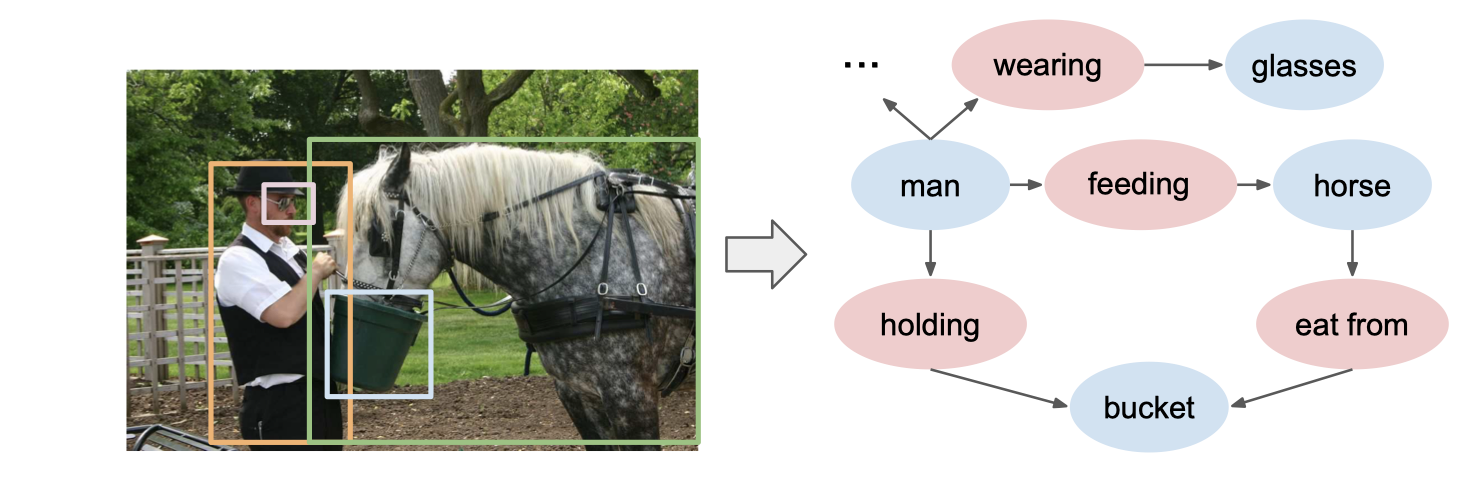
\includegraphics[width=1.0\textwidth]{figures/第二章/场景图示例.png} \\
    \bicaption[场景图示例]
    {场景图示例\cite{xu2017scene}}{Example of visual relationship dataset\cite{xu2017scene}}
   \label{场景图示例}
\end{figure}

\begin{equation}
    R(A, B) = 
    \begin{bmatrix}
        \partial A \cap \partial B & \partial A \cap B^0 & \partial A \cap B^- \\
        A^0 \cap \partial B & A^0 \cap b^0 & A^0 \cap B^- \\
        A^- \cap \partial B & A^- \cap B^0 & A^- \cap B^-
    \end{bmatrix}
\end{equation}



\section{第二节}



\section{本章小结}


% !TeX root = ../main.tex

\chapter{第三章}


% !TeX root = ../main.tex

\chapter{第四章}


% !TEX root = ../main.tex

\chapter{总结和展望}
\fancyhead[RH]{第五章\quad 总结和展望}
\section{本文工作总结}

\section{未来工作展望}

% % !TEX root = ../main.tex

\chapter{数学与引用文献的标注}

\section{数学}

\subsection{数字和单位}

宏包 \pkg{siunitx} 提供了更好的数字和单位支持:
\begin{itemize}
  \item \num{12345.67890}
  \item \num{1+-2i}
  \item \num{.3e45}
  \item \num{1.654 x 2.34 x 3.430}
  \item \si{kg.m.s^{-1}}
  \item \si{\micro\meter} $\si{\micro\meter}$
  \item \si{\ohm} $\si{\ohm}$
  \item \numlist{10;20}
  \item \numlist{10;20;30}
  \item \SIlist{0.13;0.67;0.80}{\milli\metre}
  \item \numrange{10}{20}
  \item \SIrange{10}{20}{\degreeCelsius}
\end{itemize}

\subsection{数学符号和公式}

微分符号 $\dif$ 应使用正体,本模板提供了 \cs{dif} 命令。除此之外,模板还提供了一
些命令方便使用:
\begin{itemize}
  \item 圆周率 $\uppi$:\verb|\uppi|
  \item 自然对数的底 $\upe$:\verb|\upe|
  \item 虚数单位 $\upi$, $\upj$:\verb|\upi| \verb|\upj|
\end{itemize}

公式应另起一行居中排版。公式后应注明编号,按章顺序编排,编号右端对齐。
\begin{equation}
  \upe^{\upi\uppi} + 1 = 0,
\end{equation}
\begin{equation}
  \frac{\dif^2 u}{\dif t^2} = \int f(x) \dif x.
\end{equation}

公式末尾是需要添加标点符号的,至于用逗号还是句号,取决于公式下面一句是接着公式说的,还是另起一句。
\begin{equation}
		\frac{2h}{\pi}\int_{0}^{\infty}\frac{\sin\left( \omega\delta \right)}{\omega}
		\cos\left( \omega x \right) \dif\omega = 
		\begin{cases}
				h, \ \left| x \right| < \delta, \\
				\frac{h}{2}, \ x = \pm \delta, \\
				0, \ \left| x \right| > \delta.
		\end{cases}
\end{equation}
公式较长时最好在等号“$=$”处转行。
\begin{align}
    & I (X_3; X_4) - I (X_3; X_4 \mid X_1) - I (X_3; X_4 \mid X_2) \nonumber \\
  = & [I (X_3; X_4) - I (X_3; X_4 \mid X_1)] - I (X_3; X_4 \mid \tilde{X}_2) \\
  = & I (X_1; X_3; X_4) - I (X_3; X_4 \mid \tilde{X}_2).
\end{align}

如果在等号处转行难以实现,也可在 $+$、$-$、$\times$、$\div$运算符号处转行,转行
时运算符号仅书写于转行式前,不重复书写。
\begin{multline}
  \frac{1}{2} \Delta (f_{ij} f^{ij}) =
    2 \left(\sum_{i<j} \chi_{ij}(\sigma_{i} - \sigma_{j})^{2}
    + f^{ij} \nabla_{j} \nabla_{i} (\Delta f) \right. \\
  \left. + \nabla_{k} f_{ij} \nabla^{k} f^{ij} +
    f^{ij} f^{k} \left[2\nabla_{i}R_{jk}
    - \nabla_{k} R_{ij} \right] \vphantom{\sum_{i<j}} \right).
\end{multline}

\subsection{定理环境}

示例文件中使用 \pkg{ntheorem} 宏包配置了定理、引理和证明等环境。用户也可以使用
\pkg{amsthm} 宏包。

这里举一个“定理”和“证明”的例子。
\begin{theorem}[留数定理]
\label{thm:res}
  假设 $U$ 是复平面上的一个单连通开子集,$a_1, \ldots, a_n$ 是复平面上有限个点,
  $f$ 是定义在 $U \backslash \{a_1, \ldots, a_n\}$ 上的全纯函数,如果 $\gamma$
  是一条把 $a_1, \ldots, a_n$ 包围起来的可求长曲线,但不经过任何一个 $a_k$,并且
  其起点与终点重合,那么:

  \begin{equation}
    \label{eq:res}
    \ointop_\gamma f(z)\, \dif z = 2\uppi \upi \sum_{k=1}^n \operatorname{I}(\gamma, a_k) \operatorname{Res}(f, a_k).
  \end{equation}

  如果 $\gamma$ 是若尔当曲线,那么 $\operatorname{I}(\gamma, a_k) = 1$,因此:

  \begin{equation}
    \label{eq:resthm}
    \ointop_\gamma f(z)\, \dif z = 2\uppi \upi \sum_{k=1}^n \operatorname{Res}(f, a_k).
  \end{equation}

  在这里,$\operatorname{Res}(f, a_k)$ 表示 $f$ 在点 $a_k$ 的留数,
  $\operatorname{I}(\gamma, a_k)$ 表示 $\gamma$ 关于点 $a_k$ 的卷绕数。卷绕数是
  一个整数,它描述了曲线 $\gamma$ 绕过点 $a_k$ 的次数。如果 $\gamma$ 依逆时针方
  向绕着 $a_k$ 移动,卷绕数就是一个正数,如果 $\gamma$ 根本不绕过 $a_k$,卷绕数
  就是零。

  定理~\ref{thm:res} 的证明。

  \begin{proof}
    首先,由……

    其次,……

    所以……
  \end{proof}
\end{theorem}

\section{引用文献的标注}

按照教务处的要求,参考文献外观应符合国标 GB/T 7714 的要求。模版使用 \BibLaTeX\
配合 \pkg{biblatex-gb7714-2015} 样式包
\footnote{\url{https://www.ctan.org/pkg/biblatex-gb7714-2015}}
控制参考文献的输出样式,后端采用 \pkg{biber} 管理文献。

请注意 \pkg{biblatex-gb7714-2015} 宏包 2016 年 9 月才加入 CTAN,如果你使用的
\TeX\ 系统版本较旧,可能没有包含 \pkg{biblatex-gb7714-2015} 宏包,需要手动安装。
\BibLaTeX\ 与 \pkg{biblatex-gb7714-2015} 目前在活跃地更新,为避免一些兼容性问
题,推荐使用较新的版本。

正文中引用参考文献时,使用 \verb|\cite{key1,key2,key3...}| 可以产生“上标引用的
参考文献”,如 \cite{Meta_CN,chen2007act,DPMG}。使用
\verb|\parencite{key1,key2,key3...}| 则可以产生水平引用的参考文献,例如
\parencite{JohnD,zhubajie,IEEE-1363}。请看下面的例子,将会穿插使用水平的和上标的
参考文献:关于书的\parencite{Meta_CN,JohnD,IEEE-1363},关于期刊的
\cite{chen2007act,chen2007ewi},会议论文 \parencite{DPMG,kocher99,cnproceed},硕
士学位论文\parencite{zhubajie,metamori2004},博士学位论文
\cite{shaheshang,FistSystem01,bai2008},标准文件 \parencite{IEEE-1363},技术报告
\cite{NPB2},电子文献 \parencite{xiaoyu2001, CHRISTINE1998},用户手册
\parencite{RManual}。

可以使用 \verb|\nocite{key1,key2,key3...}| 将参考文献条目加入到文献表中但不在正
文中引用。使用 \verb|\nocite{*}| 可以将参考文献数据库中的所有条目加入到文献表
中。

% % !TEX root = ../main.tex

\begin{summary}

\end{summary}


%TC:ignore

% 使用英文字母对附录编号
\appendix

% 参考文献
\newpage
\fancyhead[RH]{参考文献}
\printbibliography[heading=bibintoc]

% 附录内容
% % !TEX root = ../main.tex

\chapter{Maxwell Equations}

选择二维情况,有如下的偏振矢量:
\begin{subequations}
  \begin{align}
    {\bf E} &= E_z(r, \theta) \hat{\bf z}, \\
    {\bf H} &= H_r(r, \theta) \hat{\bf r} + H_\theta(r, \theta) \hat{\bm\theta}.
  \end{align}
\end{subequations}
对上式求旋度:
\begin{subequations}
  \begin{align}
    \nabla \times {\bf E} &= \frac{1}{r} \frac{\partial E_z}{\partial\theta}
      \hat{\bf r} - \frac{\partial E_z}{\partial r} \hat{\bm\theta}, \\
    \nabla \times {\bf H} &= \left[\frac{1}{r} \frac{\partial}{\partial r}
      (r H_\theta) - \frac{1}{r} \frac{\partial H_r}{\partial\theta} \right]
      \hat{\bf z}.
  \end{align}
\end{subequations}
因为在柱坐标系下,$\overline{\overline\mu}$ 是对角的,所以 Maxwell 方程组中电场
$\bf E$ 的旋度:
\begin{subequations}
  \begin{align}
    & \nabla \times {\bf E} = \upi \omega {\bf B}, \\
    & \frac{1}{r} \frac{\partial E_z}{\partial\theta} \hat{\bf r} -
      \frac{\partial E_z}{\partial r}\hat{\bm\theta} = \upi \omega \mu_r H_r
      \hat{\bf r} + \upi \omega \mu_\theta H_\theta \hat{\bm\theta}.
  \end{align}
\end{subequations}
所以 $\bf H$ 的各个分量可以写为:
\begin{subequations}
  \begin{align}
    H_r &= \frac{1}{\upi \omega \mu_r} \frac{1}{r}
      \frac{\partial E_z}{\partial\theta}, \\
    H_\theta &= -\frac{1}{\upi \omega \mu_\theta}
      \frac{\partial E_z}{\partial r}.
  \end{align}
\end{subequations}
同样地,在柱坐标系下,$\overline{\overline\epsilon}$ 是对角的,所以 Maxwell 方程
组中磁场 $\bf H$ 的旋度:
\begin{subequations}
  \begin{align}
    & \nabla \times {\bf H} = -\upi \omega {\bf D}, \\
    & \left[\frac{1}{r} \frac{\partial}{\partial r}(r H_\theta) - \frac{1}{r}
      \frac{\partial H_r}{\partial\theta} \right] \hat{\bf z} = -\upi \omega
      {\overline{\overline\epsilon}} {\bf E} = -\upi \omega \epsilon_z E_z
      \hat{\bf z}, \\
    & \frac{1}{r} \frac{\partial}{\partial r}(r H_\theta) - \frac{1}{r}
      \frac{\partial H_r}{\partial\theta} = -\upi \omega \epsilon_z E_z.
  \end{align}
\end{subequations}
由此我们可以得到关于 $E_z$ 的波函数方程:
\begin{equation}
  \frac{1}{\mu_\theta \epsilon_z} \frac{1}{r} \frac{\partial}{\partial r}
  \left(r \frac{\partial E_z}{\partial r} \right) + \frac{1}{\mu_r \epsilon_z}
  \frac{1}{r^2} \frac{\partial^2E_z}{\partial\theta^2} +\omega^2 E_z = 0.
\end{equation}

% % !TEX root = ../main.tex

\chapter{绘制流程图}

图~\ref{fig:flow_chart} 是一张流程图示意。使用 \pkg{tikz} 环境,搭配四种预定义节
点(\verb+startstop+、\verb+process+、\verb+decision+和\verb+io+),可以容易地绘
制出流程图。

\begin{figure}[!htp]
  \centering
  \resizebox{6cm}{!}{\input{figures/flow_chart.tex}}
  \bicaption{绘制流程图效果}{Flow chart}
  \label{fig:flow_chart}
\end{figure}

% \fancyhead[RH]{附录1}
% % !TEX root = ../main.tex
\addcontentsline{toc}{chapter}{附录}
\begin{nomenclature*}
\label{chap:symb}

\begin{longtable}{rl}
  $\epsilon$  & 介电常数  \\  
  $\mu$       & 磁导率    \\
  $\epsilon$  & 介电常数  \\
  $\mu$       & 磁导率    \\
  $\epsilon$  & 介电常数  \\
  $\mu$       & 磁导率    \\
  $\epsilon$  & 介电常数  \\
  $\mu$       & 磁导率    \\
  $\epsilon$  & 介电常数  \\
  $\mu$       & 磁导率    \\
  $\epsilon$  & 介电常数  \\
  $\mu$       & 磁导率    \\
  $\epsilon$  & 介电常数  \\
  $\mu$       & 磁导率    \\
  $\epsilon$  & 介电常数  \\
  $\mu$       & 磁导率    \\
  $\epsilon$  & 介电常数  \\
  $\mu$       & 磁导率    \\
  $\epsilon$  & 介电常数  \\
  $\mu$       & 磁导率    \\
  $\epsilon$  & 介电常数  \\
  $\mu$       & 磁导率    \\
  $\epsilon$  & 介电常数  \\
  $\mu$       & 磁导率    \\
  $\epsilon$  & 介电常数  \\
  $\mu$       & 磁导率    \\
  $\epsilon$  & 介电常数  \\
  $\mu$       & 磁导率    \\
  $\epsilon$  & 介电常数  \\
  $\mu$       & 磁导率    \\
  $\epsilon$  & 介电常数  \\
  $\mu$       & 磁导率    \\
  $\epsilon$  & 介电常数  \\
  $\mu$       & 磁导率    \\
  $\epsilon$  & 介电常数  \\
  $\mu$       & 磁导率    \\
  $\epsilon$  & 介电常数  \\
  $\mu$       & 磁导率    \\
  $\epsilon$  & 介电常数  \\
  $\mu$       & 磁导率    \\
  $\epsilon$  & 介电常数  \\
  $\mu$       & 磁导率    \\
  $\epsilon$  & 介电常数  \\
  $\mu$       & 磁导率    \\
  $\epsilon$  & 介电常数  \\
  $\mu$       & 磁导率    \\
  $\epsilon$  & 介电常数  \\
  $\mu$       & 磁导率    \\
  $\epsilon$  & 介电常数  \\
  $\mu$       & 磁导率    \\
  $\epsilon$  & 介电常数  \\
  $\mu$       & 磁导率    \\
  $\epsilon$  & 介电常数  \\
  $\mu$       & 磁导率    \\
\end{longtable}

\end{nomenclature*}


% 后文部分无编号
\backmatter



% 用于盲审的论文需隐去致谢、发表论文、科研成果、简历



% 发表论文、科研成果、简历
% 盲审论文中,发表论文及科研成果等仅以第几作者注明即可,不要出现作者或他人姓名
\newpage
\fancyhead[RH]{学术论文}
% !TEX root = ../main.tex

\begin{publications}

\end{publications}

\begin{publications*}
  
\end{publications*}

\newpage
\fancyhead[RH]{科研成果}
% !TEX root = ../main.tex


\begin{achievements*}
  \item 第一发明人,“永动机”,专利申请号XXXXXXXXXXXX.X
\end{achievements*}


% \input{contents/resume}

% 致谢
\newpage
\fancyhead[RH]{致\qquad 谢}
% !TEX root = ../main.tex

\begin{acknowledgements}

\end{acknowledgements}


% 中文学士学位论文要求在最后有一个英文大摘要,单独编页码,英文学士学位论文不需要
% % !TEX root = ../main.tex

\begin{digest}
  
\end{digest}


%TC:endignore

\end{document}